Les molécules d'un gaz peuvent être piégées à la surface d'un solide : c'est le phénomène d'adsorption. On peut distinguer deux types d'adsorption~: la chimisorption dans laquelle les molécules adsorbées forment une liaison chimique avec les atomes de la surface et l'adsorption physique dans laquelle les molécules du gaz sont liés à la surface par les forces de Van der Waals. Dans le premier type, les molécules sont adsorbées en un nombre fini de sites et forment au plus une couche monomoléculaire; dans le second type, les molécules peuvent se déposer en plusieurs couches sur la surface. Nous nous proposons d'étudier un modèle simple du deuxième type d’adsorption.

\medskip

\tiret{\'Etude de la phase gazeuse}

\smallskip

On considère tout d'abord la phase gazeuse que l'on assimile pour simplifier à un gaz 
parfait monoatomique, confiné dans un volume $V$ et à l'équilibre avec un thermostat à la température $T$. Les atomes, de masse $m$, sont supposés indiscernables et sans interactions.

\question Calculer $z(T,V)$ la fonction de partition d'un seul atome. Montrer qu'elle s'exprime comme $z(T,V)=\frac{V}{\Lambda^3}$ où $\Lambda$ est la longueur d'onde de Broglie, dont on rappellera l'expression. On donne $I_0(\alpha)=\int_{-\infty}^{+\infty} dx \ e^{-\alpha x^2}=\sqrt{\frac{\pi}{\alpha}}$.

\question En déduire la fonction de partition pour $N$ atomes $Z(T,V,N)$ en fonction de $z(T,V)$.

\question En déduire la grande fonction de partition $\Xi(T,V,\mu)$ du gaz lorsqu'il est à l'équilibre avec un réservoir au potentiel chimique $\mu$.

\question Calculer le nombre moyen $\overline{N}$ d'atomes dans la phase gaz, puis exprimer $\mu$ en fonction de $\overline{N}, V, T$ et des données.

\question Montrer que le potentiel chimique peut s'écrire: $\mu=k_B T \ln \left( \frac{P}{P_0(T)} \right)$ où $P$ est la pression du gaz et $P_0(T) \propto T^{\frac{5}{2}}.$ On pourra utiliser l'équation d'état des gaz parfaits. Exprimer $P_0(T)$.

\medskip

\tiret{Le modèle Brunauer, Emmett et Teller de la physisorption}

\smallskip

On suppose que la surface du solide sur laquelle peut se déposer les atomes comporte $M$ sites d'adsorption. Plusieurs atomes peuvent s'adsorber sur un site: on note $-\epsilon$ l'énergie de l'atome qui s'adsorbe en premier sur la surface et $-\epsilon'$ l'énergie des  atomes suivants (voir figure).
\begin{figure}[!t]
\centerline{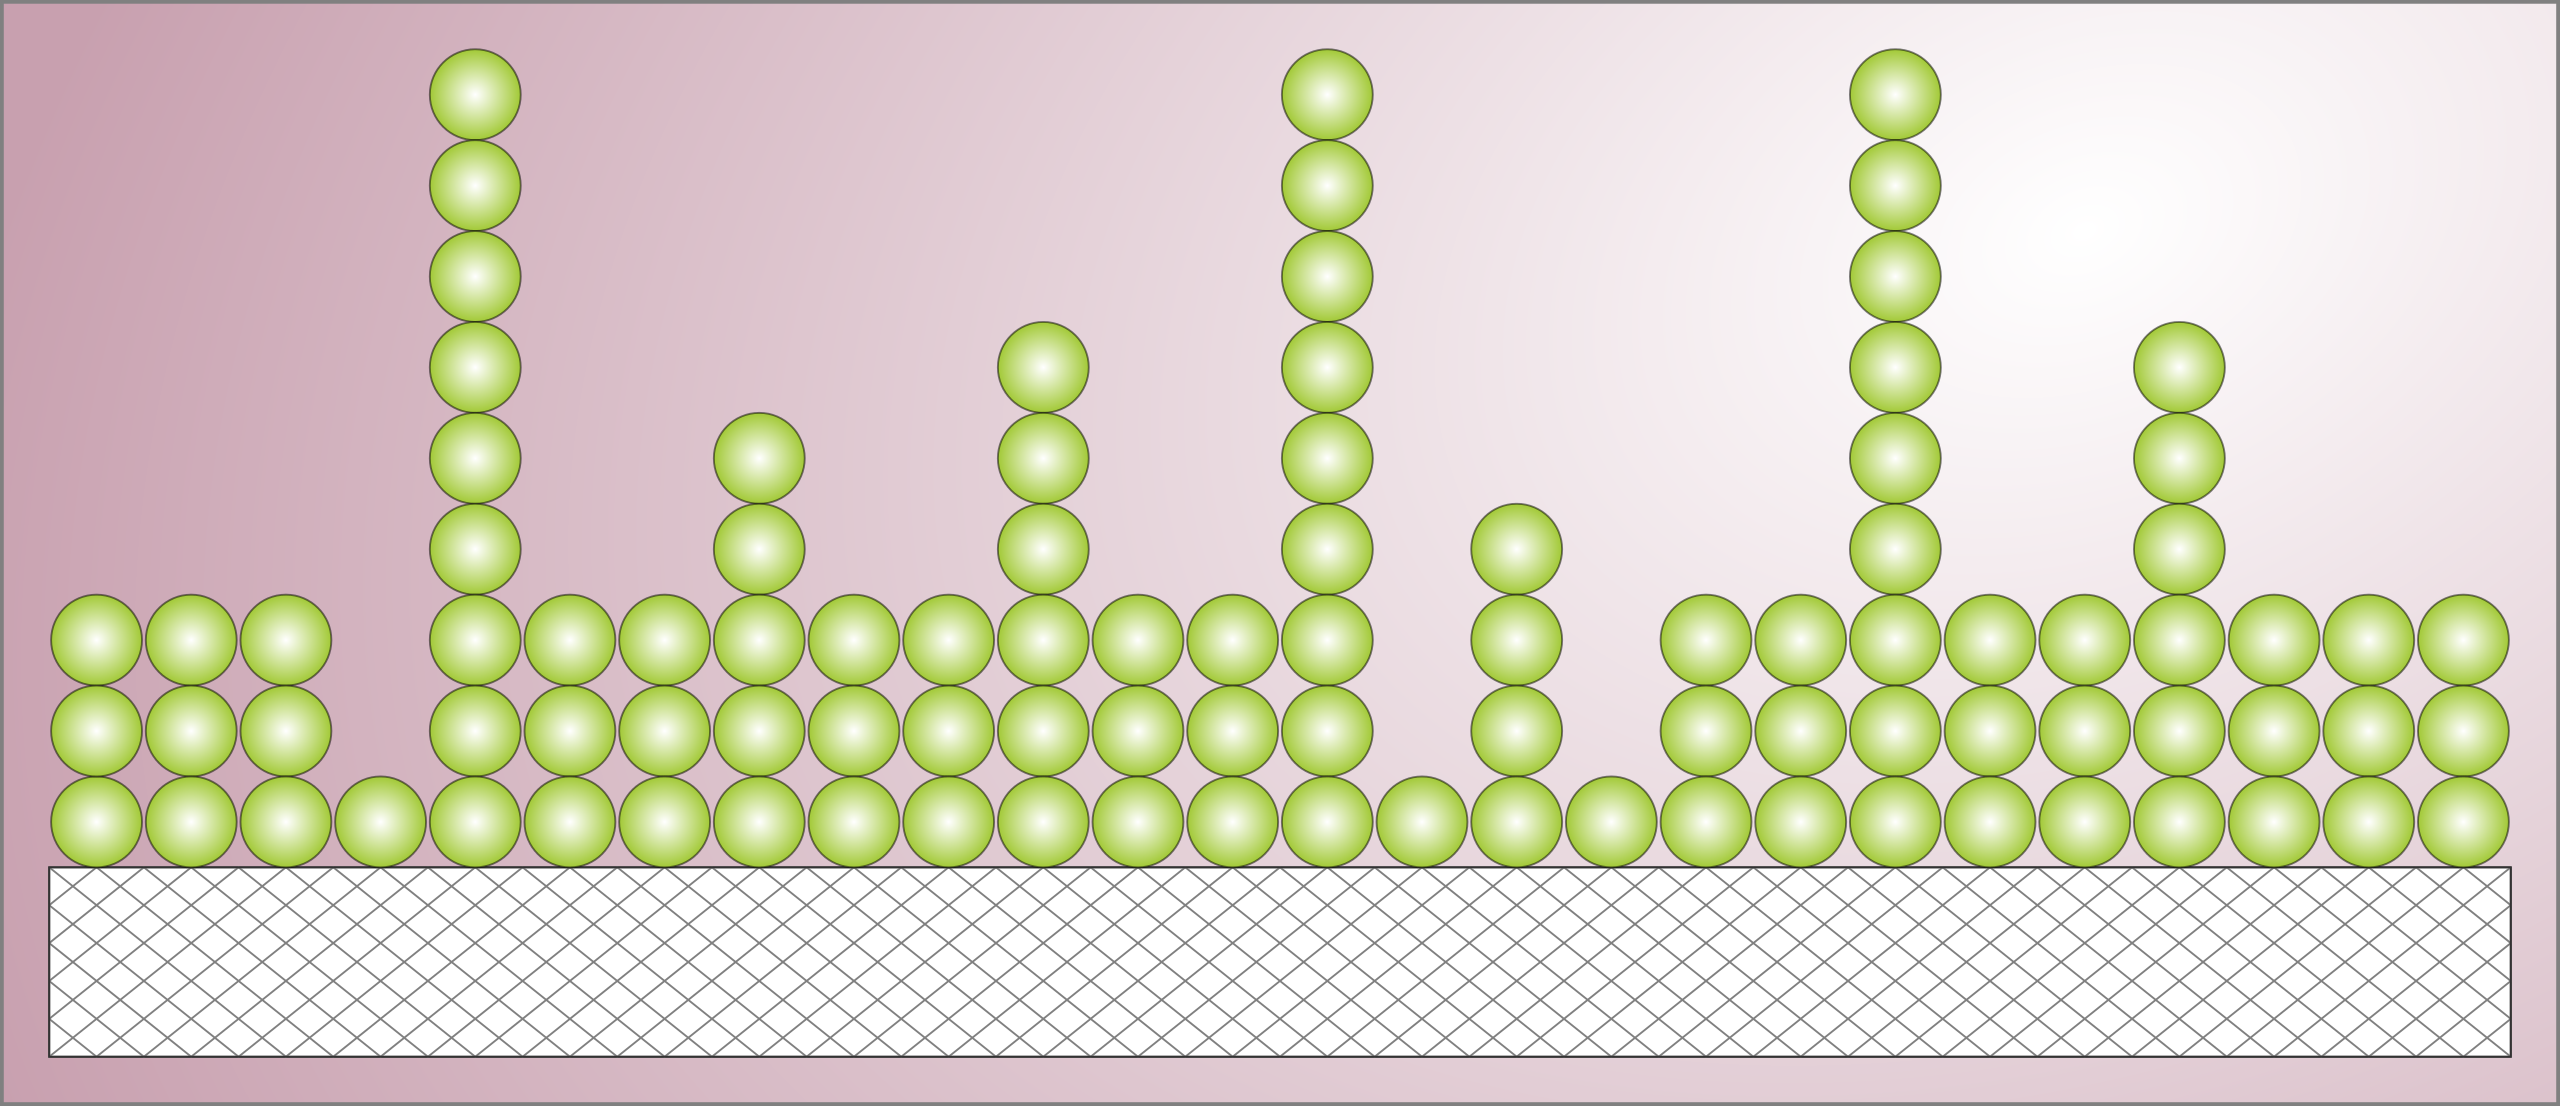
\includegraphics[height=.3\textwidth]{../Fig/BET_Multilayer_Adsorption}}
\caption{Dans le modèle BET, les atomes peuvent s'adsorber en formant des colonnes au-dessus de chaque site d'adsorption. On distingue l'énergie d'adsorption de la couche $-\epsilon$ en contact du substrat, de celles des autres couches $-\epsilon'$. Ainsi, en partant de la gauche, la première colonne (au-dessus du premier site d'adsorption) a une énergie d'adsorption $-\epsilon - 2 \epsilon'$, la quatrième $-\epsilon$, la cinquième $-\epsilon - 8 \epsilon'$. Il n'y a pas d'interactions entre atomes de colonnes différentes (c'est-à-dire adsorbés sur des sites d'adsorption différents). }
\end{figure}

\question Calculer la grande fonction de partition $\xi(T,\mu)$ d'un site d'adsorption. Montrer que, à condition que $\epsilon'+\mu<0$,  
$\xi(T,\mu)=1+\frac{b \exp(\beta \mu)}{1-b'\exp(\beta \mu)}$, où $b=\exp(\beta \epsilon)$ et $b'=\exp(\beta \epsilon')$.

\question Exprimer la grande fonction de partition $\Xi_a(T,M,\mu)$ de la phase adsorbée en fonction de $\xi(T,\mu)$.

\question En déduire le nombre moyen de particules adsorbées $\overline{N_a}$, puis le taux d'occupation de la surface $\theta=\frac{\overline{N_a}}{M}$. 

\

Le cas échéant, on peut admettre le résultat suivant: $\theta=\frac{b \exp(\beta \mu)}{[1-b' \exp(\beta \mu)][1+(b-b') \exp(\beta \mu)]}$.

\question On se place dans la limite où $b' \rightarrow 0$. Comment l'interprétez vous physiquement ? Exprimer dans cette limite $\theta$ en fonction de la pression du gaz $P$ et de $P(T)=P_0(T)/b$ uniquement. Tracer sommairement $\theta=\theta(P)$ à température fixée. Comment s'appelle cet isotherme ?

\question On introduit $c=\frac{b}{b'}$ et la pression $P'(T)=\frac{P_0(T)}{b'}$.  Exprimer $\theta$ en fonction de la pression du gaz $P$, de $c$ et $P'$ uniquement.


\question L'étude de l'adsorption de divers gaz  sur différents catalyseurs a montré que les isothermes obéissent, dans un grand domaine de pressions, à une loi de la forme:
$\frac{P}{(P'-P)V_a}=A(T)+B(T) \frac{P}{P'}$, où $V_a$ est le volume de gaz adsorbé ramené dans  les conditions normales de température et de pression. Comment relier $V_a$ à $\theta$ ? Ces résultats expérimentaux sont-ils en accord avec le modèle BET ?
